\documentclass{article}


\usepackage{arxiv}

\usepackage[utf8]{inputenc} % allow utf-8 input
\usepackage[T1]{fontenc}    % use 8-bit T1 fonts
\usepackage{hyperref}       % hyperlinks
\usepackage{url}            % simple URL typesetting
\usepackage{booktabs}       % professional-quality tables
\usepackage{amsfonts}       % blackboard math symbols
\usepackage{nicefrac}       % compact symbols for 1/2, etc.
\usepackage{microtype}      % microtypography
\usepackage{lipsum}
\usepackage{graphicx}
\graphicspath{ {./images/} }

\usepackage{amsmath}
\usepackage{amsfonts}


\title{TRUCK LOADING PROBLEM and HEURISTIC METHODS}


\author{
 Tailai Song \\
    Politecnico di Torino \\
    Corso Duca degli Abruzzi, 24 10129 TO, ITALY \\
  \texttt{s287288@studenti.polito.it} \\
   \And
 Zhiqiang Zhao \\
    Politecnico di Torino \\
    Corso Duca degli Abruzzi, 24 10129 TO, ITALY \\
  \texttt{s277962@studenti.polito.it} \\
    \And
 Di Wang \\
    Politecnico di Torino \\
    Corso Duca degli Abruzzi, 24 10129 TO, ITALY \\
  \texttt{s275509@studenti.polito.it} \\
    \And
 Yu Cheng \\
    Politecnico di Torino \\
    Corso Duca degli Abruzzi, 24 10129 TO, ITALY \\
  \texttt{s288483@studenti.polito.it} \\
}

\begin{document}
\maketitle
\begin{abstract}
This report will analyze and solve the truck loading problem through both the exact method using Gurobi and heuristic methods. Moreover, based on the comparison in terms of computational time and gap of solution, we gain a deeper understanding of operational research and more experiences in the field of applied mathematics.
\end{abstract}


% keywords can be removed
%\keywords{First keyword \and Second keyword \and More}


\section{Introduction}
\label{sec:intro}
\subsection{Introduction to the problem}
The truck loading problem states that a vehicle with $m$ compartments transports $q$ different products of various sizes from a source to $n$ different destinations. A compartment can be loaded with different products at the same time and all compartments can have the same or different capacity. The destinations have different demands for each kind of products. The demands of all the destinations must have to be satisfied all the time, which means as long as there is a lack of any kind of products at any destinations, the replenishment has to be delivered. The replenishment time is the time interval between two deliveries. The operational problem is how to load the compartments of the vehicle so that the replenishment time is maximized.
\subsection{Review of similar models} 
The family of truck loading problems, composed of many different types of loading problem branches, has been studied by many researchers. Ümit Yüceer and Arif Özakça(2010) have developed a mixed-integer linear programming model, from which they obtained weighted distribution formed sub-problems. Then the corresponding sub-algorithms and a main algorithm to limit the uncertainty interval are proposed to maximize the replenishment time. Balaji and Mukund Nilakantan(2019) studied the fixed charge transportation problem with truck load constraints (FCT-TLC) problem, and they proposed a Genetic Algorithm (GA) and a Simulated Annealing Algorithm (SAA) to minimize the cost. Maria Teresa Alonso and Ramon Alvarez-Valdes(2016) studied a truck loading problem considering the products are first loading in pallets, besides the dimension and load constraints, there are many other constraints, related to the maximum weight supported by each axle and the distribution of the load inside the truck. They have developed an improved GRASP algorithm, in which the constructive algorithm is randomized and an improvement phase is added, which including eliminating a percentage of the last trucks in the solution and refilling these trucks using another strategy, for those trucks that have been closed because an axle has reached its maximum weight, they try to obtain better results by swapping pallets between consecutive trucks so that as many pallets as possible can be loaded in the first trucks. Myrna Palmgren(2005) considered a daily transportation problem in forestry which arises when transporting logs from forest sites to customers such as sawmills and pulp and paper mills. In this problem each route has to satisfy a number of constraints concerning time windows, truck capacity, timetable of the driver, lunch breaks, etcetera, they use three solution methods based on the column generation principle, together with a pool strategy which allows them to deal with the feasible routes outside the restricted master problem.


\section{Exact solution of the Problem}
\label{sec:exact}
In order to obtain the exact solution, on one hand, it is required to derive the mathematical model and then generate instances according to the decision variables and relevant parameters. On the other hand, we use Gurobi, a computer software of mathematical optimization solver, as the exact solver.
\subsection{Mathematical model}
\paragraph{Variable definition}
$I=\{1,2,...,M\}$ is the index set of all $m$ compartments, $J=\{1,2,...,N\}$ is the index set of all $n$ destinations and $K=\{1,2,...,Q\}$ is the index set of all $q$ products.
\\$x_{ijk}$: quantity of product $k$ for destination $j$ to be loaded in compartment $i$. $i\in I, j\in J, k\in K$
\\$C_i$: the capacity of compartment $i$, $i\in I$
\\$p_k$: the size of the package of the product $k$, $k\in K$
\\$d_{jk}$: demand rate of product $k$ at destination $j$, $j\in J, k\in K$
\\$t$: replenishment time should be the minimum loading in all compartments for all products according to a certain destination.
\begin{flalign}
&t= \mathop{min}\limits_{j\in J k\in K}\{\frac{\sum _{i=1}^{M}x_{ijk}}{d_{jk}}\}&
\end{flalign}

\paragraph{Objective function}
The objective is how to load the compartments of the vehicle so that the replenishment time is maximized. We can linearize the Max-Min problem to a maximization problem with an additional constrain:
\begin{flalign}
max \ \ \ t
\end{flalign}
subject to
\begin{flalign}
&\sum_{j=1}^{N}\sum_{k=1}^{Q}p_kx_{ijk} \leq C_i \ \ \ i\in I&
\\&td_{jk} \leq \sum_{i=1}^{M}x_{ijk} \ \ \ j\in J, k \in K&
\\&x_{ijk} \geq 0, \ x_{ijk} \in \mathbb{N}^+  \ \ \ i\in I, j\in J, k \in K&
\\&t \geq 0&
\end{flalign}

\subsection{Instance generation}
To generate reasonable instances, firstly, the number of compartments $m$, the number of destinations $n$ and the number of products $q$ are fixed and can be varied manually. Secondly, $C_i$ is generated uniformly and randomly with constrains $C_L \leq C_i \textless C_H$, where $C_L$ and $C_H$ are lower limit and higher limit of the capacity of compartments, they are both assumed constant and can be modified manually. Furthermore, $p_k$ is generated in the same way, with constrains $p_L \leq p_k \textless p_H$, where $p_L$ and $p_H$ are lower limit and higher limit of the size of the packages. The demand of product $k$ at destination $j$ is denoted as $d_{j_k}$ and for each destination $j$, we generate a local limit $d_{j_L}$ and $d_{j_H}$ randomly, with constrains $0 \leq d_{j_L} \textless d_L$ and $d_{L}+1 \leq d_{j_H} \textless d_H$, then we generate $d_{j_k}$ randomly with constrains $d_{j_L} \leq d_{j_k} \textless d_{j_H}$. Note that all the parameters will be integers.

\subsection{Results based on various inputs}
We observe the various results based on modification of values in terms of compartment capacities, product sizes and demands.

\paragraph{Decreasing of compartment capacity}
In table~\ref{tab:capacity variation}, the values of objective function according to decreasing values of compartment capacity are presented and it is intuitive that  compartment capacity plays an important role in the determination of objective function result since with a less amount of capacity, the number of loading products will be less accordingly and thus, in order to satisfy the demand, we need more deliveries, in other words, higher replenishment time. 

\begin{table}[ht]
 \caption{Objective function results based on different compartment capacity}
  \centering
  \begin{tabular}{llll}
    \toprule
    Capacity of 3 compartments   & Objective function result \\
    \midrule
    810, 843, 821	&	1.25	\\
    405, 510, 410	&	0.591	\\
    270, 281, 273	&	0.391	\\
    \bottomrule
  \end{tabular}
  \label{tab:capacity variation}
\end{table}

\paragraph{Distinct product size}
The original product sizes are uniformly generated. In table~\ref{tab:size variation}, the objective function result of products with distinct sizes is shown. The second result is smaller, which means in order to have a higher replenishment time, it is suggested to avoid products that are extremely diverse in size.

\begin{table}[ht]
 \caption{Objective function results based on distinct product size}
  \centering
  \begin{tabular}{llll}
    \toprule
    Size of 3 products   & Objective function result \\
    \midrule
    20, 19, 21	&	1.25	\\
    1, 19, 40	&	1.118	\\
    \bottomrule
  \end{tabular}
  \label{tab:size variation}
\end{table}

\paragraph{Distinct demand}
According to table~\ref{tab:demand variation} , demand variation does not contribute a lot when it comes to the objective function result. Logically speaking, it is easier to satisfy the demand for product with smaller requirement by loading less amount of it, which leaves more room for others with larger demand. Consequently, the demands are fulfilled in an average way regardless the variation among products.

\begin{table}[ht]
 \caption{Objective function results based on distinct demand}
  \centering
  \begin{tabular}{llll}
    \toprule
    Demand of 3 products for 2 destinations   & Objective function result \\
    \midrule
    16, 22, 23 and 8, 17, 12	&	1.25	\\
    1, 22, 38 and 1, 17, 19	&	1.211	\\
    \bottomrule
  \end{tabular}
  \label{tab:demand variation}
\end{table}

\section{Heuristic methods}
\label{sec:heu}
Based on the review of literature and the analysis during the development, we derive two key points that can be utilized to develop heuristic methods:
\begin{itemize}
\item In order to maximize the replenishment time, we need to load products as much as possible to not only satisfy but also exceed the demands and thus, have less deliveries. It implies that we can find a feasible solution which tries to fill up all the compartments.
\item When we have a result of minimum value for a certain destination among all the replenishment time, the requirements for other destinations are also respected with higher demands. It implies that we only need to try to modify the minimum time to improve the lower limit of the requirements.
\end{itemize}

In this section we introduce three heuristic algorithms and make comparisons with exact solution.

\subsection{Partial Dynamic Programming}
\subsubsection{Introduction}
The first method we have developed is composed by two parts: 1. find a possible time that can be used to derive a feasible solution; 2. according to the value of time, try to obtain a feasible solution and at the end of each iteration, update the value of time.
\paragraph{Binary search algorithm, finding a value of time} Through this sub-algorithm, it is allowed to minimize the interval of uncertainty and further maximize the replenishment time $t$ in a fast manner. At the beginning, it is required to define the bounds, in which the lower bound $t_{lb}$ is initialized as 0, and since the maximum loading will be reached when all the rooms are filled up, so that we can consider all the compartments as a whole and therefore upper bound with relaxation is obtained by:
\begin{equation}
t_{ub} = \frac{\sum _{i=1}^{M}C_i}{\sum _{j=1}^{N}\sum _{k=1}^{Q}p_kd_{jk}}
\end{equation}
Moreover, define $t_l=(t_{lb}+t_{ub})/2$, which is used to derive a feasible solution in the following sub-algorithm. At the end of each iteration, the knowledge of feasibility will be provided. If the solution is a feasible one, which means we may still have improvement for current time $t_l$, update the lower bound with value of $t_l$. Otherwise, if the solution is infeasible, which means there's no more feasible solutions when the value of time is higher than current time, update the upper bound with $t_l$. In addition, update $t_l$ accordingly. The algorithm does not stop until the difference between bounds are smaller than a threshold of 0.03 and then output the last feasible solution.

\paragraph{Dynamic programming algorithm, find a feasible solution}
In practice, it does not matter how to load a certain product in compartments for a given destination as long as its demands has been satisfied because a destination can retrieve the same product either from, for example compartment A or compartment  B, which means we are able to only take into account the loading strategy of overall products (demand) for all destinations. As a consequence, we can derive a total product requirement based on the time provided by the previous algorithm: $D_k={\sum_{j=1}^{N}}d_{jk}t_l$. Then the problem becomes that try to find a way to load all these products in compartments. Despite the fact that there are correlations among compartments, we can still deal with compartments one by one instead of analyzing all compartments together. Therefore, for a certain compartment, we can grab products from the total quantity to try to fill it up, which resembles the classical 0-1 knapsack problem with item value being equal to item size, that can be solved by dynamic programming. And the recursive formula is:
\begin{equation}
value_{i,j} = max [value_{i-1,j}, value_{i-1,j-VS_{i,0}}+VS_{i,1}], i\in\{1,...,D\}, j\in\{1,...,C\}
\end{equation}
in which D is the total amount of all demands: $D={\sum_{k=1}^{Q}}D_k$, $C$ is the current compartment capacity, $value_{i,j}$ is the total value (total size of loaded products) at stage $i$ with occupied volume of j and VS stores the size (index 0) and value (index 1) at stage $i$. 

Now, for a compartment, we are able to find the optimal way to load products to fill the void as much as possible and we can perform the same procedure for the rest products and the next compartment. Finally, by exhausting all the compartments, if we are able to load all the products, it means there must be a feasible solution under the current condition of time. And with the output of result and feasibility, we are able to update the time bounds iteration by iteration. In conclusion, the algorithm follows the flowchart in picture \ref{fig:flowchartDP}.

\begin{figure}[ht]
    \centering
    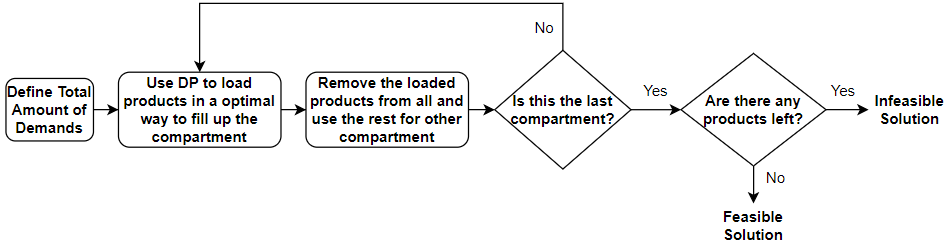
\includegraphics[scale=0.8]{flowchartDP.png}
    \caption{Flowchart for dynamic programming}
    \label{fig:flowchartDP}
\end{figure}

\subsubsection{Comparison with exact solution}
In order to evaluate the performance of this heuristic method, the gap in terms of results and computational time are taken into account.

On one hand, we have evaluated the gap with different instances generated by 200 random seeds under the same reasonable and relatively normal dimensional parameters\footnote{3 compartments, 3 products, 2 destinations, $C_L=700$, $C_H=900$, $p_L=15$, $p_H=25$, $d_L=10$, $d_H=30$ and the gap figures for all the heuristic methods are evaluated with this configuration.}. According to the histogram presented in Fig. \ref{fig:hist_pdp}, we get gaps distributing from 0\% to 1.6\% except for one and most cases are located around 0\% and 0.7\%, which indicates that the Partial Dynamic Programming method works substantially well from a statistical point of view. Although we cannot eliminate the correlation among compartments and only get a sub-optimal solution for a certain compartments, the performance is more than acceptable.

\begin{figure}[ht]
    \centering
    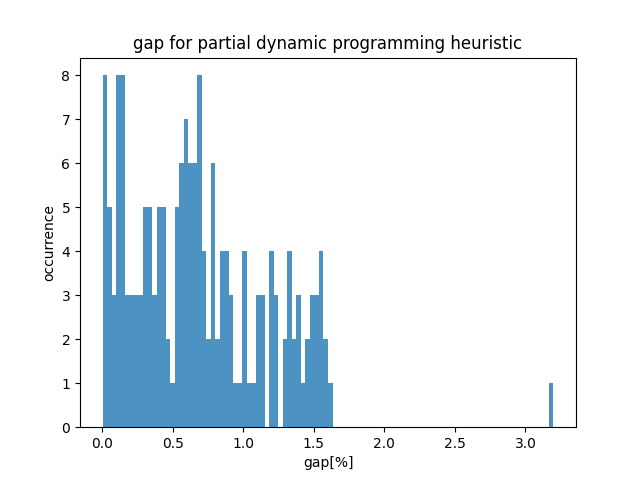
\includegraphics[scale=0.7]{hist_pdp.png}
    \caption{histogram of gap between heuristic (Partial Dynamic Programming) result and exact result for different random seeds}
    \label{fig:hist_pdp}
\end{figure}

On the other hand, we also have considered the time consumption\footnote{in some cases, it's not possible for Gurobi to derive the exact solution within seconds and the presented time are for exact solution with a gap smaller than 0.1\%.} as the dimension of parameters\footnote{changed parameters: number of products: [3, 6, 9, 12, 15], number of destinations: [2, 4, 6, 8, 10], $C_L=[700, 2800, 6300, 11200, 17500]$, $C_H=[900, 3600, 8100, 14400, 22500]$ and the rest doesn't change.} increases and the result is in Table~\ref{tab:exact_heu1}. In terms of gap, the excellent performance still holds and it has nothing to do with the complexity of the model. On contrary, the computational time increases proportionally and dramatically as the dimension of parameters increases and the values are generally unacceptable, which means it is not affordable to apply this method when we have a large scale of parameters. From a mathematical perspective, the overall time complexity is around O($mn^2\log_{}n$), which indicates that dynamic programming is not a good way to solve the problem in terms of time consumption.

\begin{table}[ht]
 \caption{Comparison of solution: Exact solver v.s Partial Dynamic Programming}
  \centering
  \begin{tabular}{llll}
    \toprule
    \multicolumn{3}{c}{Execution time}                   \\
    \cmidrule(r){2-3}
    Index   & Gurobi[s]     & PartialDP[s]      & Gap[\%] \\
    \midrule
    1	&	0.048	&	0.425	&	1.28	\\
    2	&	0.066	&	4.78	&	0.62	\\
    3	&	0.052	&	31.66	&	1.22	\\
    4	&	0.5	&	116.73	&	0.76	\\
    5	&	0.627	&	266.76	&	0.63	\\
    \bottomrule
  \end{tabular}
  \label{tab:exact_heu1}
\end{table}

\subsection{Simulation with Fair-Supply Strategy}

\subsubsection{Introduction}
Since we are dealing with a loading problem, it is also possible to derive a heuristic method to simulate the loading procedure based on a certain strategy. In particular, the goal of this problem is to increase the minimum replenishment time as much as possible, in other words, maximizing the minimum supply for the corresponding destination. Meanwhile, it is also not desirable that other non-minimum supplies are so many that occupy much more spaces and leave less for the minimum. To sum up, a strategy can be seen as a good one if we can balance the supplies for all destinations and therefore, we have developed a heuristic method based on this strategy to simulate the process. The algorithm is divided into 2 stages:
\paragraph{First stage, adding one}
We traverse all the combination of loading following the order of destination, compartment and product. In particular, For a given product required by certain destination, we add a quantity of one to the given compartment and repeat this procedure iteration by iteration until we satisfy the most basic demand for all destination in one period (t=1) or all the compartments are filled up. In addition, during this process, if a demand of a specific product required by a specific destination is met, for the following iteration, we will skip the combination of this product and destination. As a result, we give all the compartments initial occupancies satisfying the fundamental demand in an average way.
\paragraph{Second stage, adding more}
Instead of adding one item iteratively, it is more reasonable to add more items based on various demands since a higher demand requires a higher supply to increase the related replenishment time. Therefore, in this stage, we still follow the traversal process but with a increment of a product to a compartment varying according to its the demand. The increment can be determined by the ratio of corresponding demand divided by the minimum demand of all products for a certain destination, e.g. we use the minimum as a base, a Carrefour store needs 2 kg apples, 6 kg bananas and 10 kg oranges, then the increment (supply) should be 2/2=1 kg apples, 6/2=3 kg bananas and 10/2=5 kg oranges. In addition, if a compartment cannot hold a certain product with a specific increment anymore, we decrease the increment by one until the increment reaches one, which means this compartment is full. In the previous stage, we satisfy the demand in an average way while in this stage, we increase the supply (demand) in an average manner. 

In the end, we stop the simulation when all compartments are full and by averaging the product demand, we balance not only the distribution of products in compartments but also all the supplies to avoid penalizing a certain destination.

\subsubsection{Comparison with exact solution}
The comparison has been done in the same way with respect to the previous method. 

In Fig. \ref{fig:hist_so}, obviously, the performance in terms of gap is worse than the previous method but with relatively acceptable results ranging from 0\% to 6\%. Moreover, there exist few gaps with value greater than 10\% and up to 20\% due to some instances with large variation in demands, which means this method doesn't perform well versatilely.

\begin{figure}[ht]
    \centering
    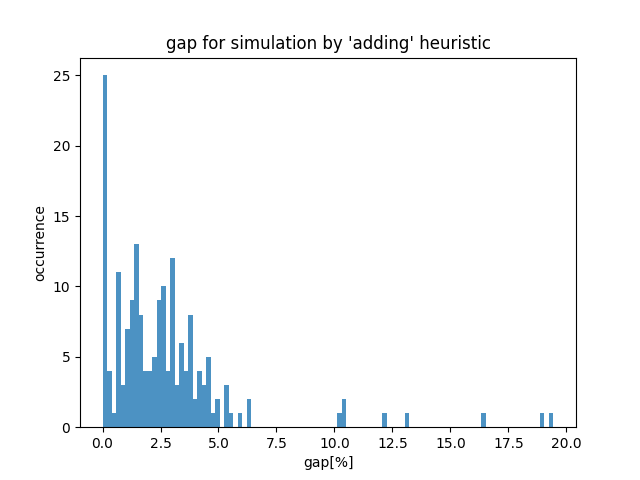
\includegraphics[scale=0.7]{hist_so.png}
    \caption{histogram of gap between heuristic (Simulation with Fair-Supply Strategy) result and exact result for different random seeds}
    \label{fig:hist_so}
\end{figure}

Being different from the performance for gaps, Table \ref{tab:exact_heu2} demonstrates a huge improvement when it comes to the computational time. As the increasing of complexity, the time consumption doesn't increase with a large amount but it cannot be ignored that the gap is still an issue.

\begin{table}[ht]
 \caption{Comparison of solution: Exact solver v.s Partial Dynamic Programming}
  \centering
  \begin{tabular}{llll}
    \toprule
    \multicolumn{3}{c}{Execution time}                   \\
    \cmidrule(r){2-3}
    Index   & Gurobi[s]     & PartialDP[s]      & Gap[\%] \\
    \midrule
    1	&	0.048	&	0.001	&	5.45	\\
    2	&	0.066	&	0.025	&	2.12	\\
    3	&	0.052	&	0.353	&	7.41	\\
    4	&	0.5	&	1.82	&	1.72	\\
    5	&	0.627	&	6.67	&	4.88	\\
    \bottomrule
  \end{tabular}
  \label{tab:exact_heu2}
\end{table}

\subsection{Simulation with greedy algorithm}

\subsubsection{Introduction}
Referring to the Value Independent Knapsack Problem which is also called Subset-sum Problem(SSP), the most immediate and efficient approach for the heuristic solution is the greedy algorithm, which consists in examining the products in any order and inserting each new item into the compartment if it fits. This heuristic method also has two sub-algorithms in which the first one is the same as in partial dynamic programming and generate a value of time for the next sub-algorithm to process.

In the second sub-algorithm with greedy method, all products for corresponding supply (demand) that ought to be loaded are sorted by size in descending order, which means we are giving the large product a priority. First of all, starting from one destination, the compartments are filled with products one by one until all required products for this destination are loaded or the compartments have too little space to fit any more products. Secondly, the products of next destination will be chosen to fill up the compartments until all destinations have been examined. In the end, after the greedy loading process, a feasible solution can be accessed if all the demands are satisfied, in other words, compartments are filled up with all the products. Otherwise, the output feasibility will be negative. Simply put, we are trying to derive a voracious loading strategy to load products as much as possible with feasibility check at the end. A flowchart is presented in Fig.\ref{fig:flowchartgreedy}.

\begin{figure}[ht]
    \centering
    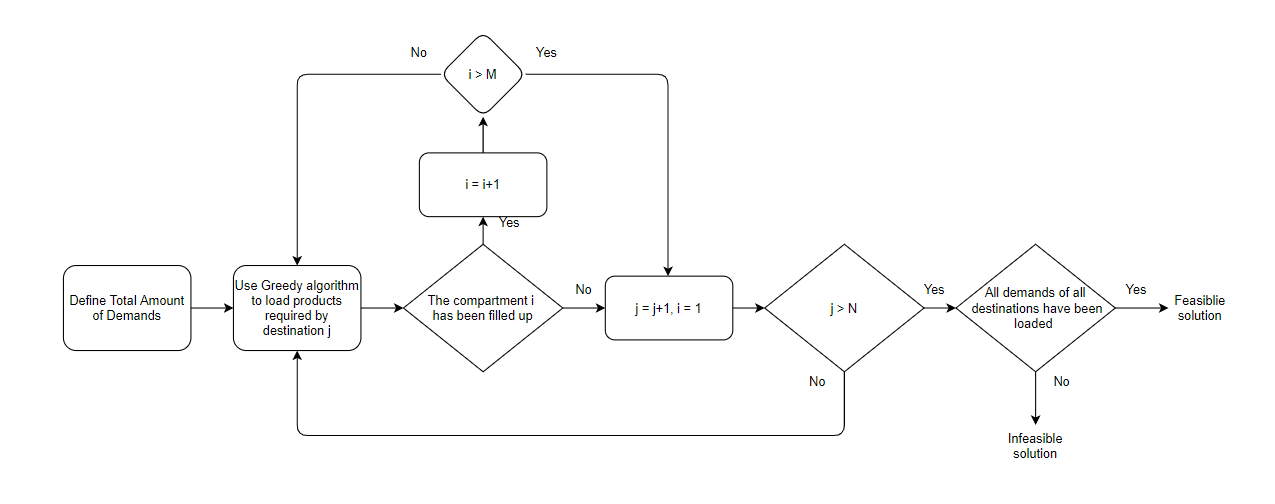
\includegraphics[scale=0.6]{flowchartgreedy.png}
    \caption{Flowchart for simulation with greedy algorithm}
    \label{fig:flowchartgreedy}
\end{figure}

\subsubsection{Comparison with exact solution}
The same comparisons have been proceeded and results are presented in Fig.\ref{fig:hist_sg} and Table.\ref{tab:exact_greedy}. In terms of gaps, there is a huge amount of gaps with value of 0\%, which means it is possible to reach a extremely precise result with respect to the exact solution, but the distribution of other gaps is relatively dispersive indicating a unstable performance. On top of that, the time consumption is so small that can be ignored, even for a high complexity, which results in a hegemony in heuristic method choice if the computational time is the paramount consideration. It is mainly due to the fact that the total time complexity is only O($n\log_{}n$).

\begin{figure}[ht]
    \centering
    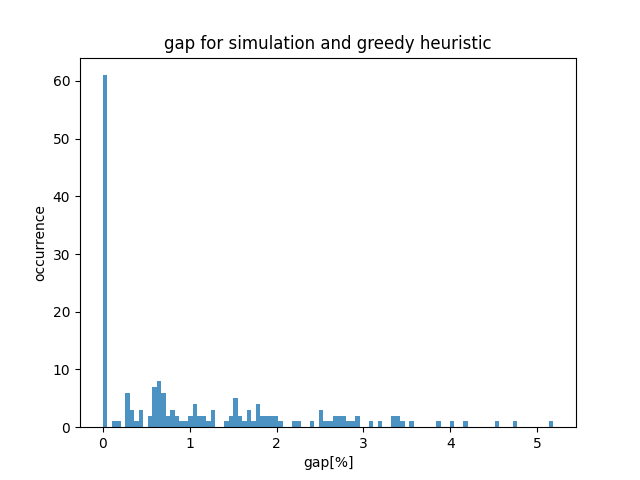
\includegraphics[scale=0.7]{hist_sg.png}
    \caption{histogram of gap between heuristic (Simulation with greedy algorithm) result and exact result for different random seeds}
    \label{fig:hist_sg}
\end{figure}

\begin{table}[ht]
 \caption{Comparison of solution: Exact solver v.s Simulation with greedy algorithm}
  \centering
  \begin{tabular}{llll}
    \toprule
    \multicolumn{3}{c}{Execution time}                   \\
    \cmidrule(r){2-3}
    Index   & Gurobi[s]     & greedy[s]      & Gap[\%] \\
    \midrule
    1	&	0.048 	&	0.001 	&	0.00 	\\
    2	&	0.066 	&	0.002 	&	0.00 	\\
    3	&	0.052 	&	0.002 	&	0.97 	\\
    4	&	0.498 	&	0.004 	&	0.41 	\\
    5	&	0.627 	&	0.004 	&	0.35 	\\
    \bottomrule
  \end{tabular}
  \label{tab:exact_greedy}
\end{table}

\subsection{Summary of heuristic methods}
The ultimate goal is to find a fast and good heuristic method to solve the truck loading problem. Besides the comparison between certain heuristic method and the exact solver, the worst case performance is indeed an important indicator when it comes to the evaluation of heuristic methods. Furthermore, a general comparison taking into account all the factors, among all the heuristic methods can be conducted to draw a conclusion.

\subsubsection{Worst case analysis}
To begin with, four relatively extreme scenarios with different parameters are considered. All the results in the following are derived based on instances generated by 100 different random seeds but with certain parameters being fixed. In addition, two kinds of results are presented: 1. number of times when a certain heuristic method gives the highest objective function result among all three. Note that there might be more than one heuristic methods providing same highest value; 2. average gap with respect to exact solver.

\paragraph{Distinct compartment capacity}
The fixed parameter in this section is the compartment capacity with very distinct values: 200, 800 and 1400. Consequently, all the heuristic methods have to deal with the fact that the loading conditions in different compartments are more correlated. Table.\ref{tab:distinct compartment capacity for heu} shows the results and apparently, the second heuristic method, simulation with fair supply, gives the worst performance while the other two perform similarly with good average gap. Additionally, compartment capacity variation makes little contribution in generation of a worse result with respect to exact solver since the overall volume is still adequate, and the opposite condition will be presented in the end.

\begin{table}[ht]
 \caption{Comparison in terms of distinct compartment capacity for all heuristic methods}
  \centering
  \begin{tabular}{llll}
    \toprule
    \multicolumn{3}{c}{Values}                   \\
    \cmidrule(r){2-3}
    description   & Partial DP    & Simulation with fair-supply      & Simulation with greedy \\
    \midrule
    highest result occurrence[-]	&	42 	&	17 	&	55 	\\
    average gap[\%]	&	0.65 	&	3.22 	&	0.88 	\\
    \bottomrule
  \end{tabular}
  \label{tab:distinct compartment capacity for heu}
\end{table}

\paragraph{Distinct product size}
The product sizes of 1, 20 and 39 are the key parameters in this section. Technically speaking, a product with small volume can be loaded easily and thus, the corresponding demand can be respected with less constrains. But for a large-volume product, loading one more quantity will consume much more spaces. This strong characteristic of variation will play a crucial role in heuristic method decision making. According to Table.\ref{tab:distinct product size for heu}, simulation of greedy algorithm provides the best solution and dominates in both criteria. In addition, partial dynamic programming still has a good average gap but cannot provide accurate results, which means it works in a stable and mediocre manner. 

\begin{table}[ht]
 \caption{Comparison in terms of distinct product size for all heuristic methods}
  \centering
  \begin{tabular}{llll}
    \toprule
    \multicolumn{3}{c}{Values}                   \\
    \cmidrule(r){2-3}
    description   & Partial DP    & Simulation with fair-supply      & Simulation with greedy \\
    \midrule
    highest result occurrence[-]	&	19 	&	31 	&	76	\\
    average gap[\%]	&	0.84	&	2.41 	&	0.49 	\\
    \bottomrule
  \end{tabular}
  \label{tab:distinct product size for heu}
\end{table}

\paragraph{Distinct demand}
We keep the demands for both destination:1, 10, 35 and 1, 15, 30 as fixed parameters. Obviously, a higher demand requires more supplies which indicates that the improvement of replenishment time for this destination is hard to be made and the product supplies are difficult to be balanced. As we can see in Table.\ref{tab:distinct demand for heu}, this case penalize more than the previous two especially for the second heuristic method. Simulation with greedy algorithm still gives the best performance while partial dynamic programming is also acceptable.

\begin{table}[ht]
 \caption{Comparison in terms of distinct demand for all heuristic methods}
  \centering
  \begin{tabular}{llll}
    \toprule
    \multicolumn{3}{c}{Values}                   \\
    \cmidrule(r){2-3}
    description   & Partial DP    & Simulation with fair-supply      & Simulation with greedy \\
    \midrule
    highest result occurrence[-]	&	37 	&	0	&	64	\\
    average gap[\%]	&	0.997	&	17.2 	&	0.872 	\\
    \bottomrule
  \end{tabular}
  \label{tab:distinct demand for heu}
\end{table}

\paragraph{Relatively small compartment capacity}
As mentioned in the first section, smaller volume for compartment with respect to size of products will lead to that loading just one more quantity of product may be impossible. In other word, the increment of products into compartments is with small magnitude, which may result in a huge difference between the result of heuristic method and exact solver. In this section, the lower bound and upper bound of compartment capacity for generating instances are fixed: 100 and 200\footnote{the lower bound and upper bound of product size are 15 and 25, it's hard to load a lot of products in a compartment with volume from 100 to 200}. And just like what has been anticipated, according to Table.\ref{tab:small compartment capacity for heu}, this condition affect heuristic methods the most. Simulation with fair supply is out of the game with absolutely unacceptable results while the other two work similarly.

\begin{table}[ht]
 \caption{Comparison in terms of small compartment capacity for all heuristic methods}
  \centering
  \begin{tabular}{llll}
    \toprule
    \multicolumn{3}{c}{Values}                   \\
    \cmidrule(r){2-3}
    description   & Partial DP    & Simulation with fair-supply      & Simulation with greedy \\
    \midrule
    highest result occurrence[-]	&	45 	&	1	&	56	\\
    average gap[\%]	&	4.26	&	40.1 	&	4.42 	\\
    \bottomrule
  \end{tabular}
  \label{tab:small compartment capacity for heu}
\end{table}

\subsubsection{Summary}
At this point, we have completed the comparison in various ways and it is possible to draw several specific conclusions.

\begin{itemize}
\item The second heuristic method, simulation with fair supply has to be dropped because: 1. it provides neither the least time consumption nor the smallest value for gap; 2. worst cases affect it too much to be accepted.
\item The other two methods, partial dynamic programming and simulation with greedy algorithm are both performing very well in terms of gap no matter it is normal evaluation or worst case analysis.
\item Partial dynamic programming works in a more stable way with less variance, but as the complexity of model grows, the time consumption becomes an inevitable issue and cannot be avoided due to intrinsic property.
\item Simulation with greedy algorithm performs decently from both perspectives of statistical value and time complexity, but the stability has to be considered.
\end{itemize}

\section{Conclusion }
To begin with, through the comprehensive study and thorough analysis of the truck loading problem, we are eventually able to derive heuristic methods to acquire solutions without referring to the exact solver. In general, all the methods posted above provide potentially acceptable and reasonable results but one of them does not perform well enough especially when it comes to the worst scenarios. Meanwhile, the other two work with pro and con that can be further optimized. In particular, partial dynamic programming has a steady behaviour while simulation with greedy algorithm is much more efficient. 

However, there is still a key point of truck loading problem that can be easily ignored, which is that just by loading or unloading \textbf{one} product, the optimized result of minimum replenishment time will be modified by a very small quantity since in most cases, one product does not contribute a lot with respect to the overall demand or supply. In other words, the difference between the optimized result and its consecutive sub-optimized result is too small with a tiny magnitude to be considered. Hence, although it is true that the result of these heuristic methods are acceptable from a statistical point of view, a decrement of, for example 0.1\% (which may represent a numerous number of products) in gap, can be actually considered as a huge improvement. For this reason, partial dynamic programming with a stable performance may be a better heuristic method even it is computationally expensive.

Moreover, it is obvious that for a time sensitive application with a high complexity, partial dynamic programming cannot be adopted. And simulation with greedy algorithm will play its dominant role in this region. Given the fact that as the dimension of parameters increases, Gurobi cannot even provide exact result and proceed for hours, this heuristic method is more significant, not to mention that the results are also acceptable.

In conclusion, on one hand, since we are focusing on finding a good and fast heuristic method, simulation with greedy algorithm is the best one as a whole. On the other hand, referring to partial dynamic programming if time consumption is irrelevant. 

\bibliographystyle{unsrt}  

\begin{thebibliography}{1}

\bibitem{2010}
Ümit Yüceer \& Arif Özakça. (2010). 
\newblock A truck loading problem. Computers \& Industrial Engineering 58, 766–773.

\bibitem{2019}
A. N. Balaji, J. Mukund Nilakantan, Izabela Nielsen, N. Jawahar \& S. G. Ponnambalam (2019).
\newblock Solving fixed charge transportation problem with truck load constraint using metaheuristics. Annals of Operations Research 273, 207–236.

\bibitem{2016}
Maria Teresa Alonso, Ramon Alvarez-Valdes, Francisco Parreño \& Jose Manuel Tamarit. (2016).
\newblock Algorithms for Pallet Building and Truck Loading in an Interdepot Transportation Problem. Mathematical Problems in Engineering, 2016, Article ID 3264214.

\bibitem{2005}
Myrna Palmgren (2005).
\newblock Optimal Truck Scheduling: Mathematical Modeling and Solution by the Column Generation Principle. Linköping University.

\bibitem{1990}
Martello,S.,\&Toth,P. (1990).
\newblock Knapsack problems: Algorithms and computer implementations. New York:John Wiley \& Sons.

\end{thebibliography}


\end{document}
